\documentclass[12pt,a4paper]{report}
\newcommand{\mychapter}[2]{
    \setcounter{chapter}{#1}
    \setcounter{section}{0}
    \chapter*{#2}
    \addcontentsline{toc}{chapter}{#2}
}
\let\EndItemize\enditemize
\def\enditemize{\EndItemize\bigskip}
\setlength{\headheight}{15pt} 
\usepackage[utf8]{inputenc}
\usepackage{amsmath}
\usepackage{graphicx}
\usepackage[colorinlistoftodos]{todonotes}
\usepackage[T1]{fontenc}
\usepackage[french]{babel}
\usepackage{courier}
\usepackage{listings}
\usepackage{float}
\usepackage{epigraph}
\usepackage{fancyhdr}
\usepackage[xindy]{glossaries}
\makeglossaries
\pagestyle{fancy}

\fancyhead[R,L]{\fontsize{8}{15}\thepage}
\fancyhead[L]{\slshape\nouppercase{\rightmark}}
\fancyhead[R]{\slshape\nouppercase{\leftmark}}
\title{Cahier des charges}

\date{\today}

\newcommand{\hsp}{\hspace{20pt}}
\newcommand{\HRule}{\rule{\linewidth}{0.5mm}}

\lstdefinestyle{base}{
  language=C,
  emptylines=1,
  breaklines=true,
  basicstyle=\ttfamily\color{black},
  moredelim=**[is][\color{mygreen}]{@}{@},
  moredelim=**[is][\color{blue}]{µ}{µ},
  moredelim=**[is][\color{blue}]{~}{~},
  showstringspaces=false
}
\lstdefinestyle{algo}{
  morekeywords={algorithme,procedure,si,fin,alors,variables,sinon,debut},
}

\begin{document}

\begin{titlepage}
  \begin{sffamily}
  \begin{center}


    \textsc{Rapport de première soutenance}\\[1.5cm]

	
\includegraphics[scale=0.04]{logo-epita.png}~\\[1.5cm]
    
    % Title
    \HRule \\[0.4cm]
    { \huge \bfseries A2C\\[0.4cm] }
    \HRule \\[1cm]
    % Ici notre logo
    %\\[1cm]

       {Team \textsc{MALT (anciennement Ghom)} \\
        Promo 2018}\\[1.5cm]

        Thibaud "zehir" Michaud \\
	    Lucien "Luciano" Boillod \\
        Charles "Arys" Yaiche \\
        Maxime "Kylox" Gaudron

    \vfill
	{\large 10 Janvier 2014}

  \end{center}
  \end{sffamily}
\end{titlepage}

\tableofcontents
\newpage

\mychapter{0}{Introduction}

Le projet A2C est un compilateur du langage Algo vers le langage C, qui a pour but de faciliter leur enseignement dans les classes préparatoires d'EPITA.
La team MALT s'est assez naturellement formée avant le début du quatrième semestre, étant tous redoublant dû au semestre international. Notre projet étant assez ambitieux pour des étudiants de SPE, la phase de documentation a été une étape importante et nécessaire avant toute implémentation.
On a donc emprunté des ouvrages de référence dans le domaine comme "Modern Compiler Implementation" ou encore "Compiler: Principles, Techniques and Tools (aka Dragon Book) afin d'acquérir une compréhension générale sur les compilateurs et la théorie des langages. Deux d'entre nous ont d'ailleurs eu la chance d'assister aux cours de THL d'ING1 durant leur stage au LRDE du S3, ce qui leur a permis d'assimiler les premières notions importantes. \\

Ce rapport détaille le travail effectué depuis la naissance du projet. Nous verrons que ce dernier a bien avancé, et a même dépassé nos objectifs initiaux.
Dans un premier temps nous décrivons notre organisation, puisque la team a tenu à ce qu'elle soit exemplaire afin d'éviter de gros rush inutiles.

\mychapter{1}{Organisation}
\section{Organisation du groupe}
Avant même le début du S4, nous avons commencé à se réunir afin de discuter de l'organisation du projet, ce qui a permis de mettre en place rapidement des outils de développpement (GIT, intégrateur continu ...), un workflow avec des rôles attitrés (intégrateur de GIT, Chef de projet ...), et une réunion hebdomadaire.
Nous avons ainsi tenté de rester serieux tout au long de cette première période en instaurant cette réunion obligatoire le lundi soir. Ce qui nous a poussé à travailler régulièrement et à s'assurer qu'il y avait une bonne communication et une bonne entente entre les membres du groupe.
Au programme de ces réunions: un rappel de ce qui à été fait depuis la dernière réunion, un échange et une explication si nécessaire de nos parties, un point sur ce qu'il reste à faire avec l'écriture du TODO.
Ce mode de fonctionnement était très efficace puisque à l'issu de la réunion chacun repartait avec un objectif pour la semaine d'après.

\section{Organisation du projet}
\subsection{Chronologie}
La chronologie définie dans le cahier des charges a du être revue au cours de la réalisation du projet. Nous avions segmenté le projet en trop gros blocs : parseur, génération de code, etc. et nous nous sommes rendu compte que nous ne pourrions pas travailler comme ça car tant qu'une tâche n'est pas finie, les autres sont bloquées et ne peuvent pas avancer. \\

Nous sommes donc repartis dans l'idée de commencer par un langage très simple constitué uniquement d'expressions arithmétiques, et de travailler sur toute les parties du projet en même temps à partir de ce langage. L'idée étant ensuite d'étendre le langage au fur et à mesure jusqu'à atteindre le langage algo. \\

Cette organisation s'est avérée très efficace. Nous avons ainsi pu travailler tous en même temps, et nous avions tout de suite des résultats satisfaisants malgré la simplicité du langage. Nous avons ensuite pu compléter le langage assez facilement, si bien que nous avons dépassé nos objectifs. \\

\subsection{Le parseur}
Nous avions prévu d'écrire le parseur à la main. Nous gardons en tête cette idée, mais nous avons pour l'instant décidé d'utiliser les générateurs de lexeur/parseur flex et bison. La raison est simple : toujours dans l'idée de pouvoir travailler sur toutes les parties du projet en même temps, il fallait écrire le parseur au plus vite. Ainsi nous avons déjà pu commencer la génération de code et l'analyse sémantique. Ces deux dernières tâches étant indépendantes
du parseur en lui même et ne reposant que sur l'arbre syntaxique abstrait, il sera facile à l'avenir de réécrire le parseur sans compromettre ce qui a déjà été fait.

\mychapter{2}{Travail Effectué}
% detailler par section
\section{Ecriture de la grammaire du langage}
Cette première partie permet de délimiter le langage Algo et de mieux comprendre son fonctionnement, et ainsi pouvoir faire les rapprochement avec le langage C. Nous avons donc repris le mémo en ligne contenant toutes les spécifications du langage et commencant à écrire la grammaire abstraite. Elle nous a également familiarisé avec la grammaire du langage et son type (Hors contexte), ce qui nous a révélé les ambiguités et les difficultés auquelles nous seront confrontés. \\

Des questions ont été posé à Nathalie sur certains points qui pouvait être interprété de différentes manières ou alors qui n'était pas spécifié, afin de ne pas prendre trop de liberté sur la syntaxe et l'utilisation et de coller le plus possible au langage initial.

Il a été ainsi question de l'ordre de déclaration des paramètres, les expressions comme les char, le passage de pointeur à certaines fonctions comme lire ... 

Nous avons essayé dès le début de définir tous les cas possibles afin de couvrir tout le langage et identifier les cas qui pourrait poser problème.

Nous nous sommes également inspiré de l'interpréteur de Marwan Burelle, pour certaines choses qui n'étaient pas défini dans le langage comme les variables globales, ou le point d'entrée principale d'un programme.
\newpage

\section{Structures de données}
Nous avons réfléchi avant de  commencer les autres tâches aux éventuelles structures de données dont nous pourrions avoir besoin, et les avons implémentées. La plupart des structures devaient être génériques, afin de pouvoir servir dans plusieurs parties à la fois. Voici les structures implémentées jusqu'ici :\\

\begin{itemize}
\item liste statique / pile
\item table de hachage
\end{itemize}

Nous avons d'abord implémenté les structures basiques comme des listes chainées, nous avions pensé à des listes intrusives, mais au final, de simples listes statiques nous ont semblé plus intéréssantes. Nous avons fait le choix d'implémenter ces listes sous forme de macro pour gérer la généricité. 

La table de hachage servira surtout pour la table de symboles. La généricité a été gérée de la même manière que pour les listes, avec des macros. les collisions sont gérées par chainage, l'ajout se fait en tête et non en queue. Ainsi, lorsqu'un contexte local est défini avec une collision de symbole par rapport à un contexte global, la valeur récupérée dans la table de symbole correspondra au symbole local.\\


\newpage

\section{Lexeur/Parseur}
Comme expliqué précedemment, nous avons décidé d'utiliser flex et bison pour écrire le parseur. Ce n'est qu'une solution temporaire car nous espérons recoder le parseur à la main, cependant il se peut que cette solution devienne permanente si le temps nous manque pour faire le reste du projet d'ici les prochaines soutenances. \\

Pour le parseur nous nous sommes beaucoup documenté, car même en utilisant un générateur de parseur, l'écriture d'une grammaire sans ambiguités et sans conflits n'est pas immédiate. Certains membres du groupe ont assisté aux cours de THL d'ING1 (ce qui a été une des sources d'inspiration à l'origine du projet) et nous avons consulté les ouvrages de référence tels que "Compilers: Principles Techniques and Tools" et "Modern Compiler Implementation in ML". \\

Nous sommes d'abord partis d'une grammaire très simple reconaissant des expressions arithmétiques entières. Nous avons ensuite étendu cette grammaire aux différents types : caractères, booléens, etc. Puis sont venues les instructions : assignations, appels de fonction et structures conditionnelles. Enfin, nous avons ajouté la définition d'une fonction, la déclaration des variables et le point d'entrée du programme.

Pour construire le langage, nos principales références étaient
\begin{itemize}
\item La page dédiée à la syntaxe du langage algo sur le site infoprepa.epita.fr (http://algo.infoprepa.epita.fr/index.php/Epita:Algo:M%C3%A9mo-Langage)
\item L'interpréteur epi-algo de Marwan (https://code.google.com/p/epi-algo/)
\end{itemize}

\newpage

\section{Ecriture de l'arbre syntaxique abstrait}
L'arbre syntaxique abstrait est le point d'articulation d'un compilateur. Il représente la syntaxe du programme fourni en entrée et permet ensuite d'analyser et de manipuler ce programme sur une structure de donnée simple et intuitive plutôt que sur du texte brut. C'est le rôle du parseur de générer cet arbre. \\

Un arbre syntaxique est, de par sa nature, abstrait. Il est difficile à représenter dans un langage bas niveau tel que le C et se représente plus facilement dans un langage qui supporte la généricité. \\

Par exemple un noeud de l'arbre doit représenter une expression. Une expression peut prendre de nombreuses formes (deux expressions liées par un opérateur binaire, déréférencement d'un pointeur, accès à l'élément d'un tableau, etc.). Pour représenter ce polymorphisme nous avons représenté ce noeud comme une struct contenant :
\begin{itemize}
\item Une enum indiquant le type d'expression dont il s'agit.
\item Une union pouvant contenir tous les types d'expression possibles.
\end{itemize}
Ainsi lorsqu'on parcours l'arbre et que l'on tombe sur un noeud expression, il suffit de regarder l'enum pour savoir de quel type d'expression il s'agit, puis d'aller chercher la valeur de cette expression dans l'union en fonction du type d'expression. \\

Voici pour illustrer le code qui affiche un expression de type "2 expressions liées par un opérateur binaire" :


\begin{figure}[H]
  \begin{lstlisting}[style=base]
  void print_expression(struct expr *e)
  {
    switch (e->exprkind)
    {
      (...)
      case binopexprkind:
        printf("(");
        print_expression(e->val.binopexpr.e1);
        printf(" %s ", getopstr(e->val.binopexpr.op));
        print_expression(e->val.binopexpr.e2);
        printf(")");
        break;
      (...)
    }
  }
  \end{lstlisting}
  \caption{extrait de la fonction print\_expression}
  \label{print_binop}
\end{figure}

Les opérateurs binaires sont représentés par leur numéro de token (défini par bison), et la fonction getopstr se charge de traduire ce numéro en une chaîne de caractère correspondant au bon opérateur.

\newpage

\section{Analyse de type}
L'analyse de type est une étape importante dans la compilation, elle fait partie d'une plus grande partie nommée l'analyse sémantique. Elle consiste à vérifier la bonne consistance des types dans les expressions des diverses instructions. Les plus simples a vérifier sont les opérations unaires et binaires sur des entiers et booléens directement.
Nous nous sommes d'abord penchés sur ces cas dans le but de présenter une compilation d'un sous langage du langage algo, qui contient uniquement des assignation de variable et des opérations unaires et binaires, comme une sorte de calculatrice  basique.

\subsection{Les instructions}
L'analyse de type d'une expression utilise les struct "instruction" comprises dans la structure de l'algo. 
Pour vérifier les instructions il nous faut d'abord récuperer son type, s'il s'agit d'une boucle "pour", une boucle "tant que" ou autre.
\begin{itemize}
\item boucle : pour les boucles il suffit de vérifier la condition et toute les expressions la composant
\item assignation : verification du type a gauche et a droite de l'assignation.
\end{itemize}

\subsection{Les expressions}
Pour réaliser cette étape il nous suffit donc simplement de parcourir l'AST en sortie du parseur. Chaque noeud possédant leur type dans leur structure il nous est alors facile de verifier la validité de l'expresion
\begin{itemize}
\item binop : il suffit de verifier que l'opérateur agit sur des types entier, reel ou booléen et que le type de l'expression gauche est le même que celui de droite.
\item unop :  même chose que pour une binop on a juste pas besoin de vérifier le type d'expression à gauche. 
\end{itemize}
Il s'agit donc donc basiquement d'un parcours profondeur de l'ast.
\subsection{Conclusion}
L'analyse de type a attendu la fin de la conception de l'ast qui a beaucoup bougé durant toute cette première période et pourra donc être finalisé pour la soutenance 2. Cependant une structure basique d'analyse de type a été implémenté, et nous avons déjà réfléchi à da conception ce qui permettra une implémentation rapide dans le futur.
\newpage

\section{Génération de code}
Une fois l'AST construit, la génération de code est assez simple à implémenter. En effet, le langage algo étant assez proche du C, il suffit de parcourir récursivement l'arbre syntaxique et d'afficher pour chaque noeud le code C correspondant. (cf fig. \ref{print_binop}). \\

Certains cas ne peuvent pas être gérés aussi simplement. Notamment en ce qui concernent les symboles prédéfinis. La table des symboles n'est pas encore implémentée, et une fonction prédéfinie telle que "écrire" en algo est transcodée telle quelle en C alors qu'il faudrait détécter le symbole et écrire "puts" en oubliant pas d'inclure <stdio.h> dans le fichier généré. Voici un exemple de traduction :\\

\begin{figure}[h]
\begin{tabular}{|c|c|}
  \begin{lstlisting}[style=algo]
algorithme procedure affiche_42
variables
  entier a, b
  reel c
debut
  a <- 12
  si (a > 10) alors
    a <- a + 30
  sinon
    a <- a - 10
  fin si
  ecrire(a)
fin algorithme procedure affiche_42

variables
debut
  affiche_42()
fin
  \end{lstlisting}
  &
  \begin{lstlisting}[style=base]
void affiche_42(void)
{
  entier a, b;
  reel c;
  a = 12;
  if ((a > 10))
  {
    a = (a + 30);
  }
  else
  {
    a = (a - 10);
  }
  ecrire(a);
}
int main(void)
{
  affiche_42();
}

  \end{lstlisting}
\end{tabular}
\label{exemple}
\caption{exemple de traduction}
\end{figure}

Pour l'instant ce code C est généré sur la sortie standard. C'est à l'utilisateur de décider ce qu'il en fait.

\newpage

\section{Site Web}
Le site web reste quelque chose d'important dans tout projet, car il est en quelque sorte sa vitrine.
On voulait quelque chose de simple, épuré mais qui reste classe qui n'est pas seulement un index html.
Le site web doit également être un vecteur de communication efficace entre les développpeurs et les utilisateurs ou encore les développeurs du projet avec des développeurs externes, cest pour ça que nous avons défini une section communauté, qui contient  les liens de contact aussi bien vers nos adresses mails que vers nos comptes github, les bug reports, ainsi qu'une section concernant les contributions et les demandes de merge du projet pour ceux qui voudrait se joindre à l'aventure !
Un section pour la documentation est également présente, bien que non écrite encore.
Bien sûr des news sont postées régulièrement, pour prévenir des différentes versions et des bugs, ainsi qu'une section de téléchargement des sources du projet.
\newline
\newline

\begin{figure}[H]
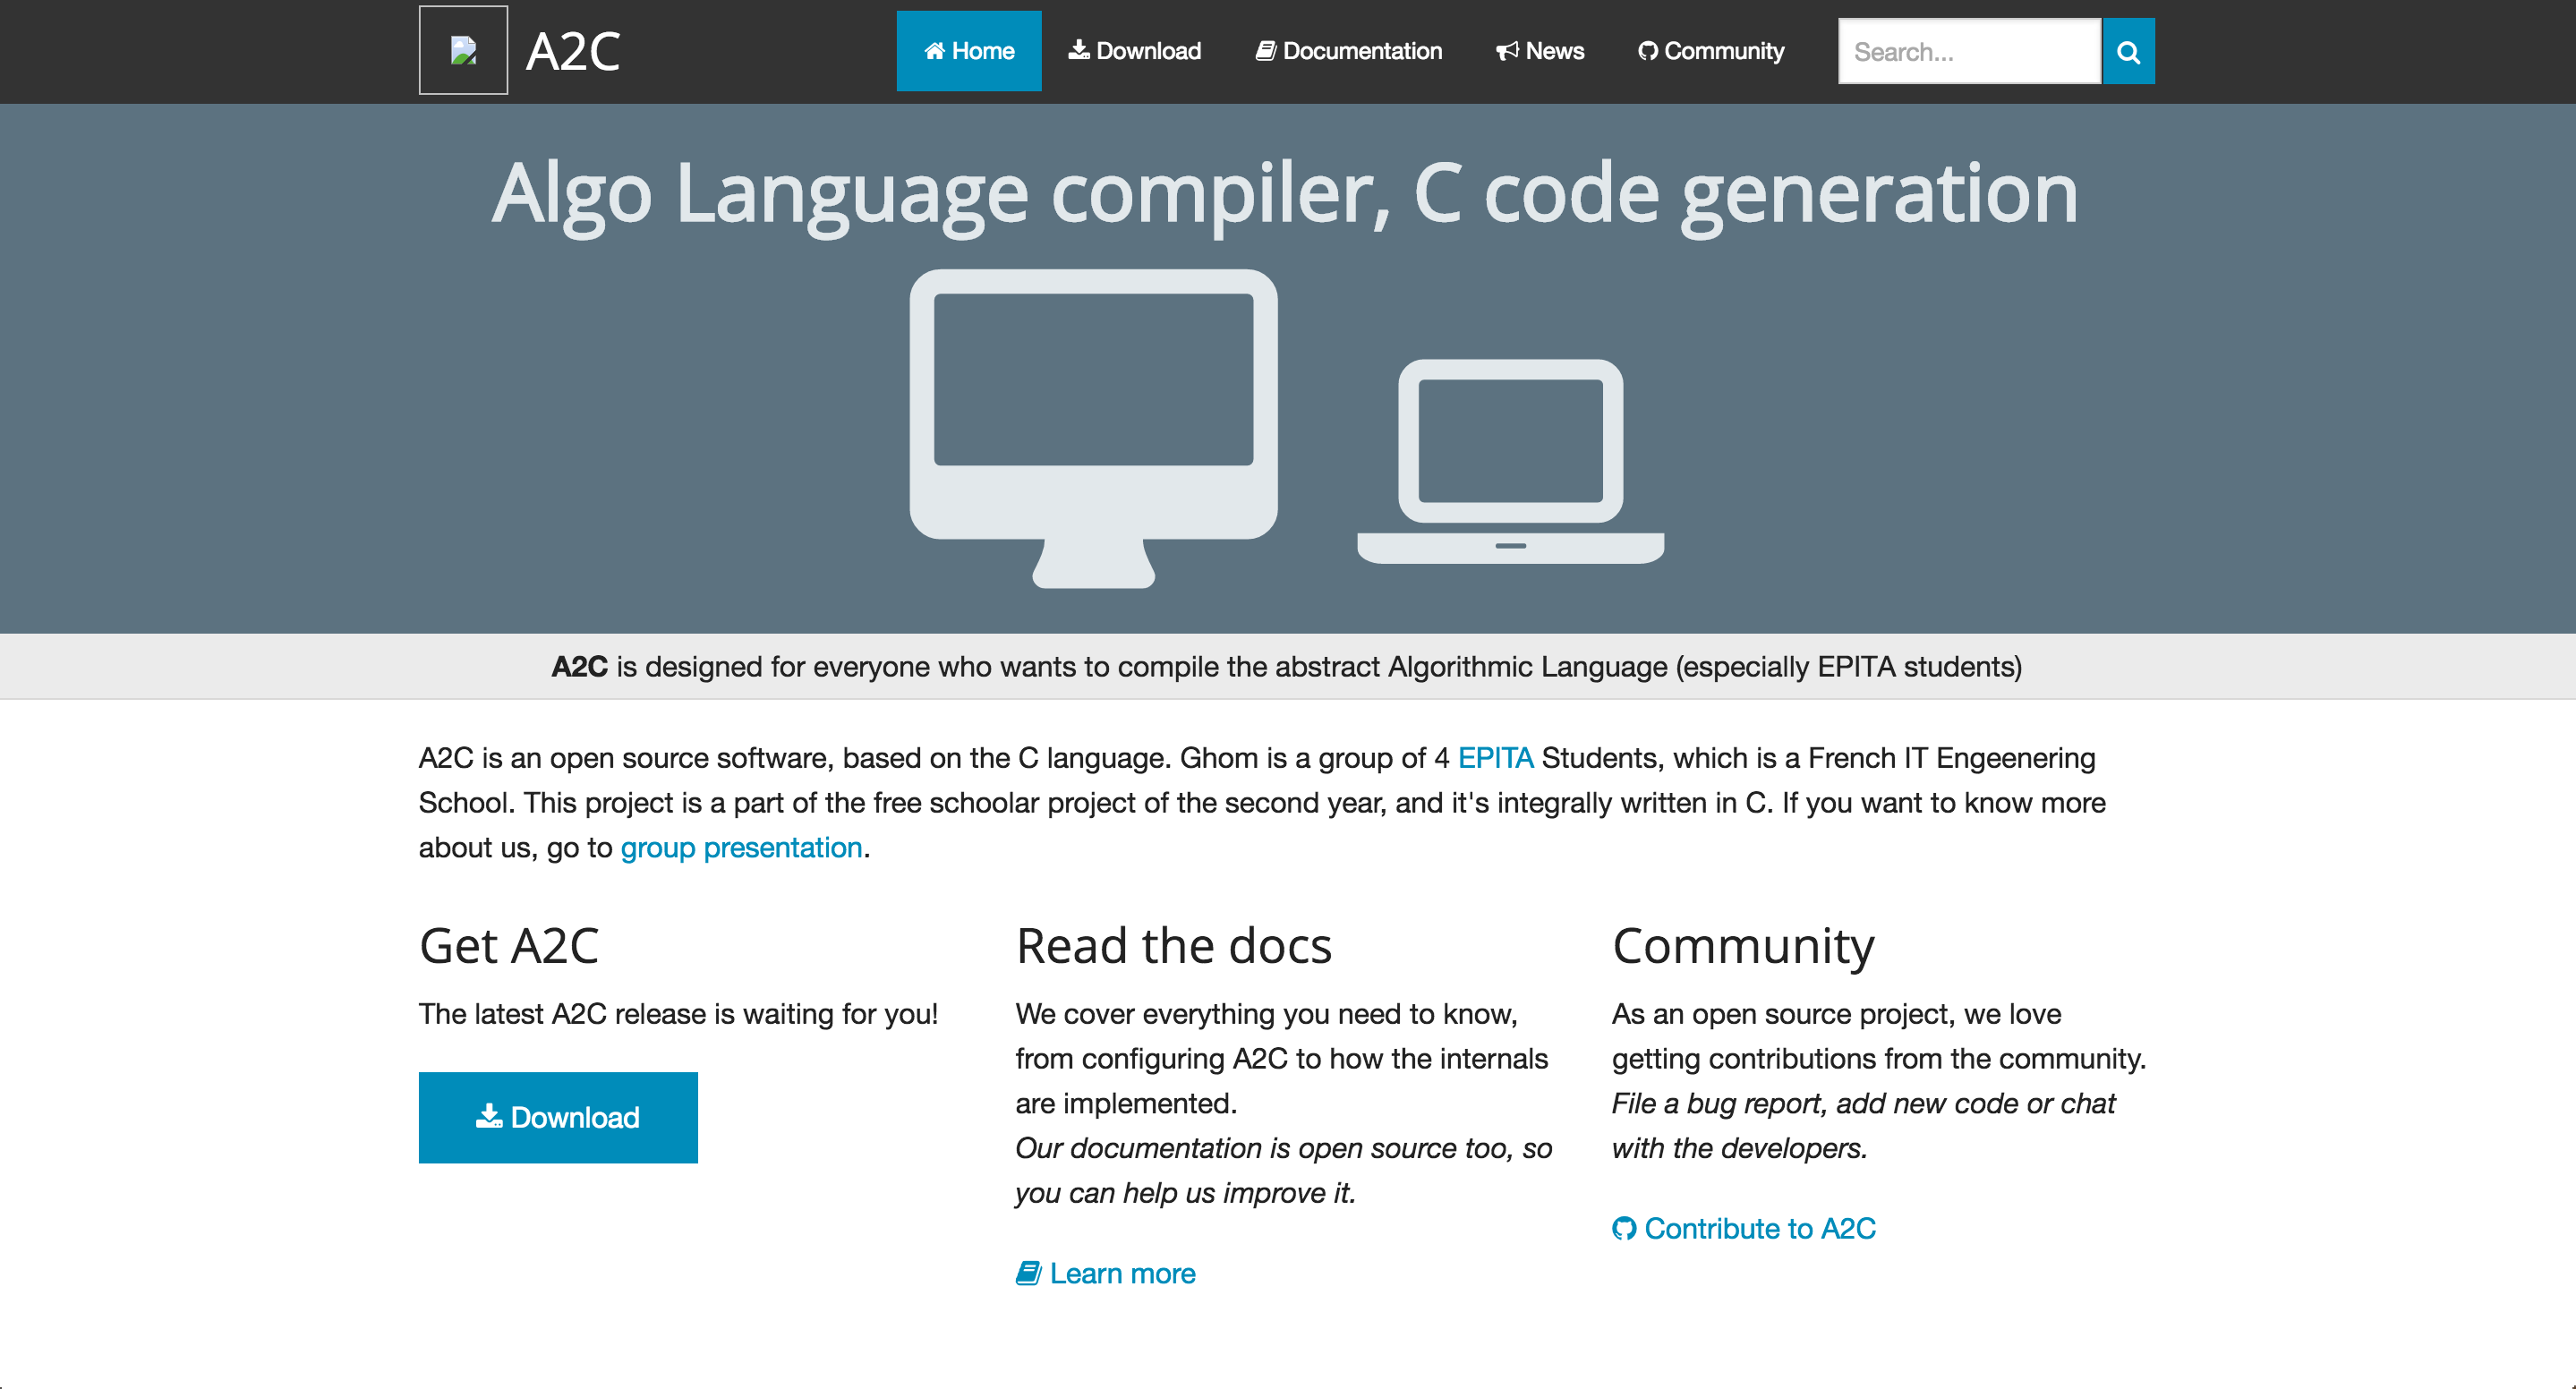
\includegraphics[scale=0.2]{website.png}~\\[1.5cm] \\
\caption{Accueil du site}
\end{figure}
\begin{figure}[H]
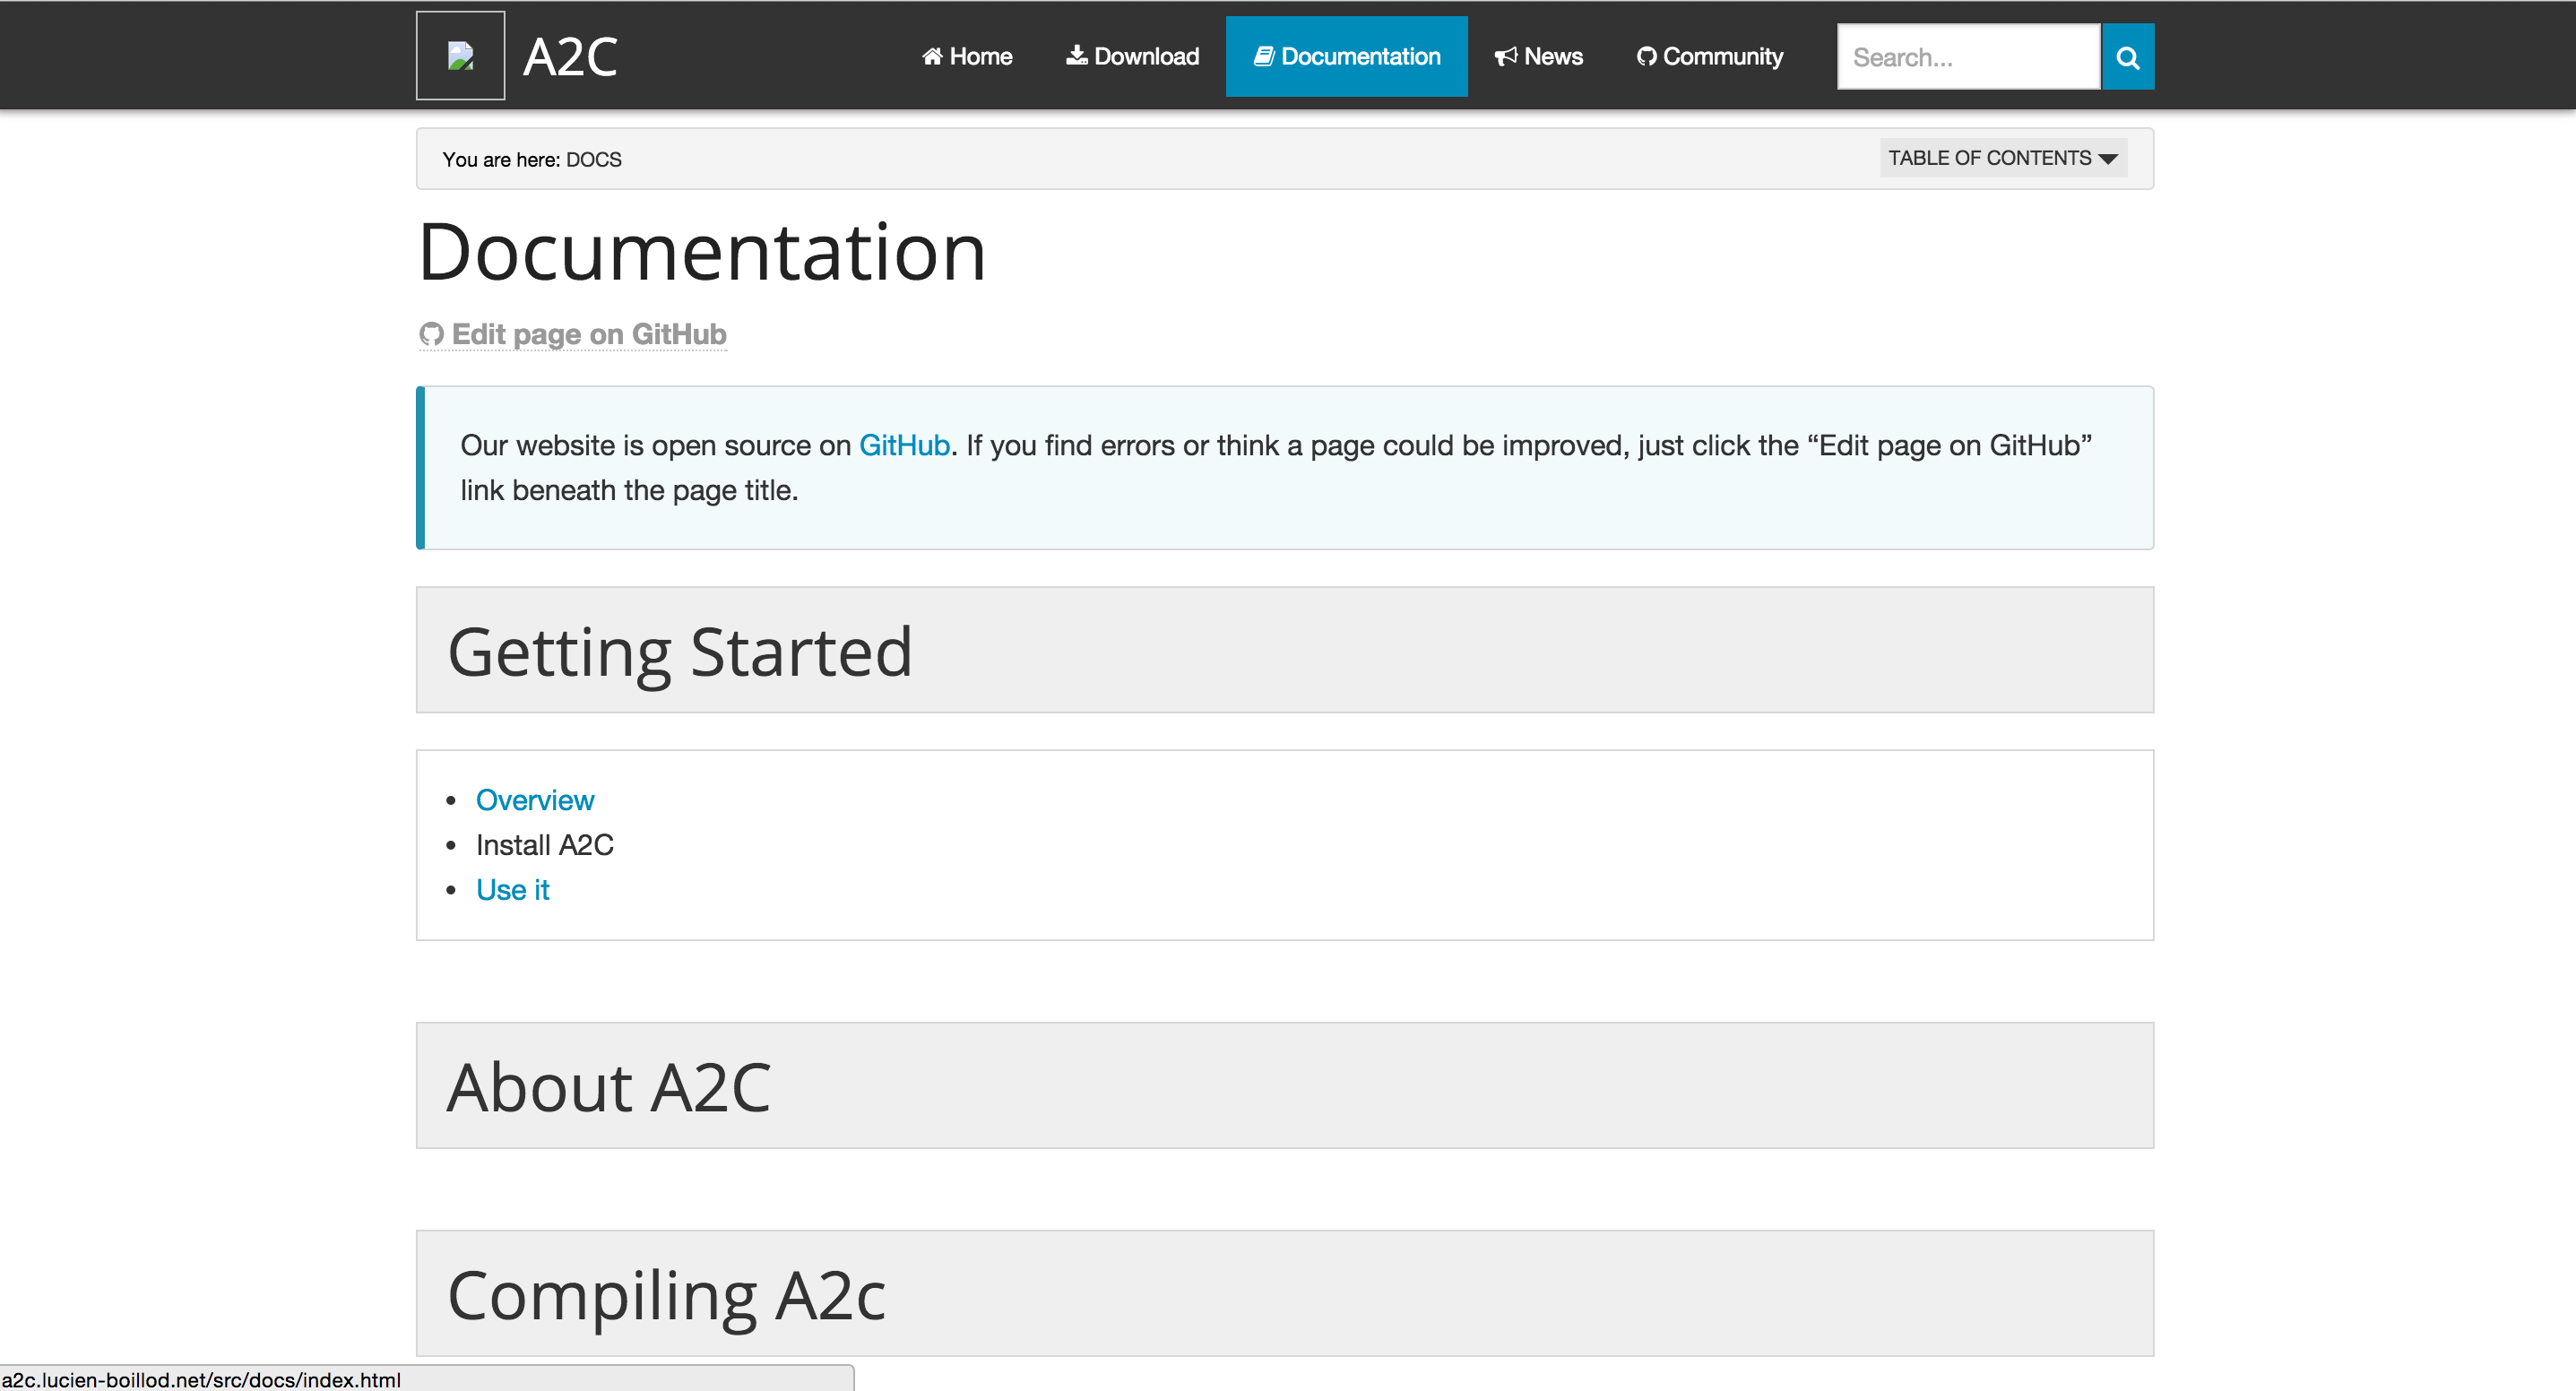
\includegraphics[scale=0.2]{website2.png}~\\[1.5cm] \\
\caption{Wiki du projet}
\end{figure}\begin{figure}[H]
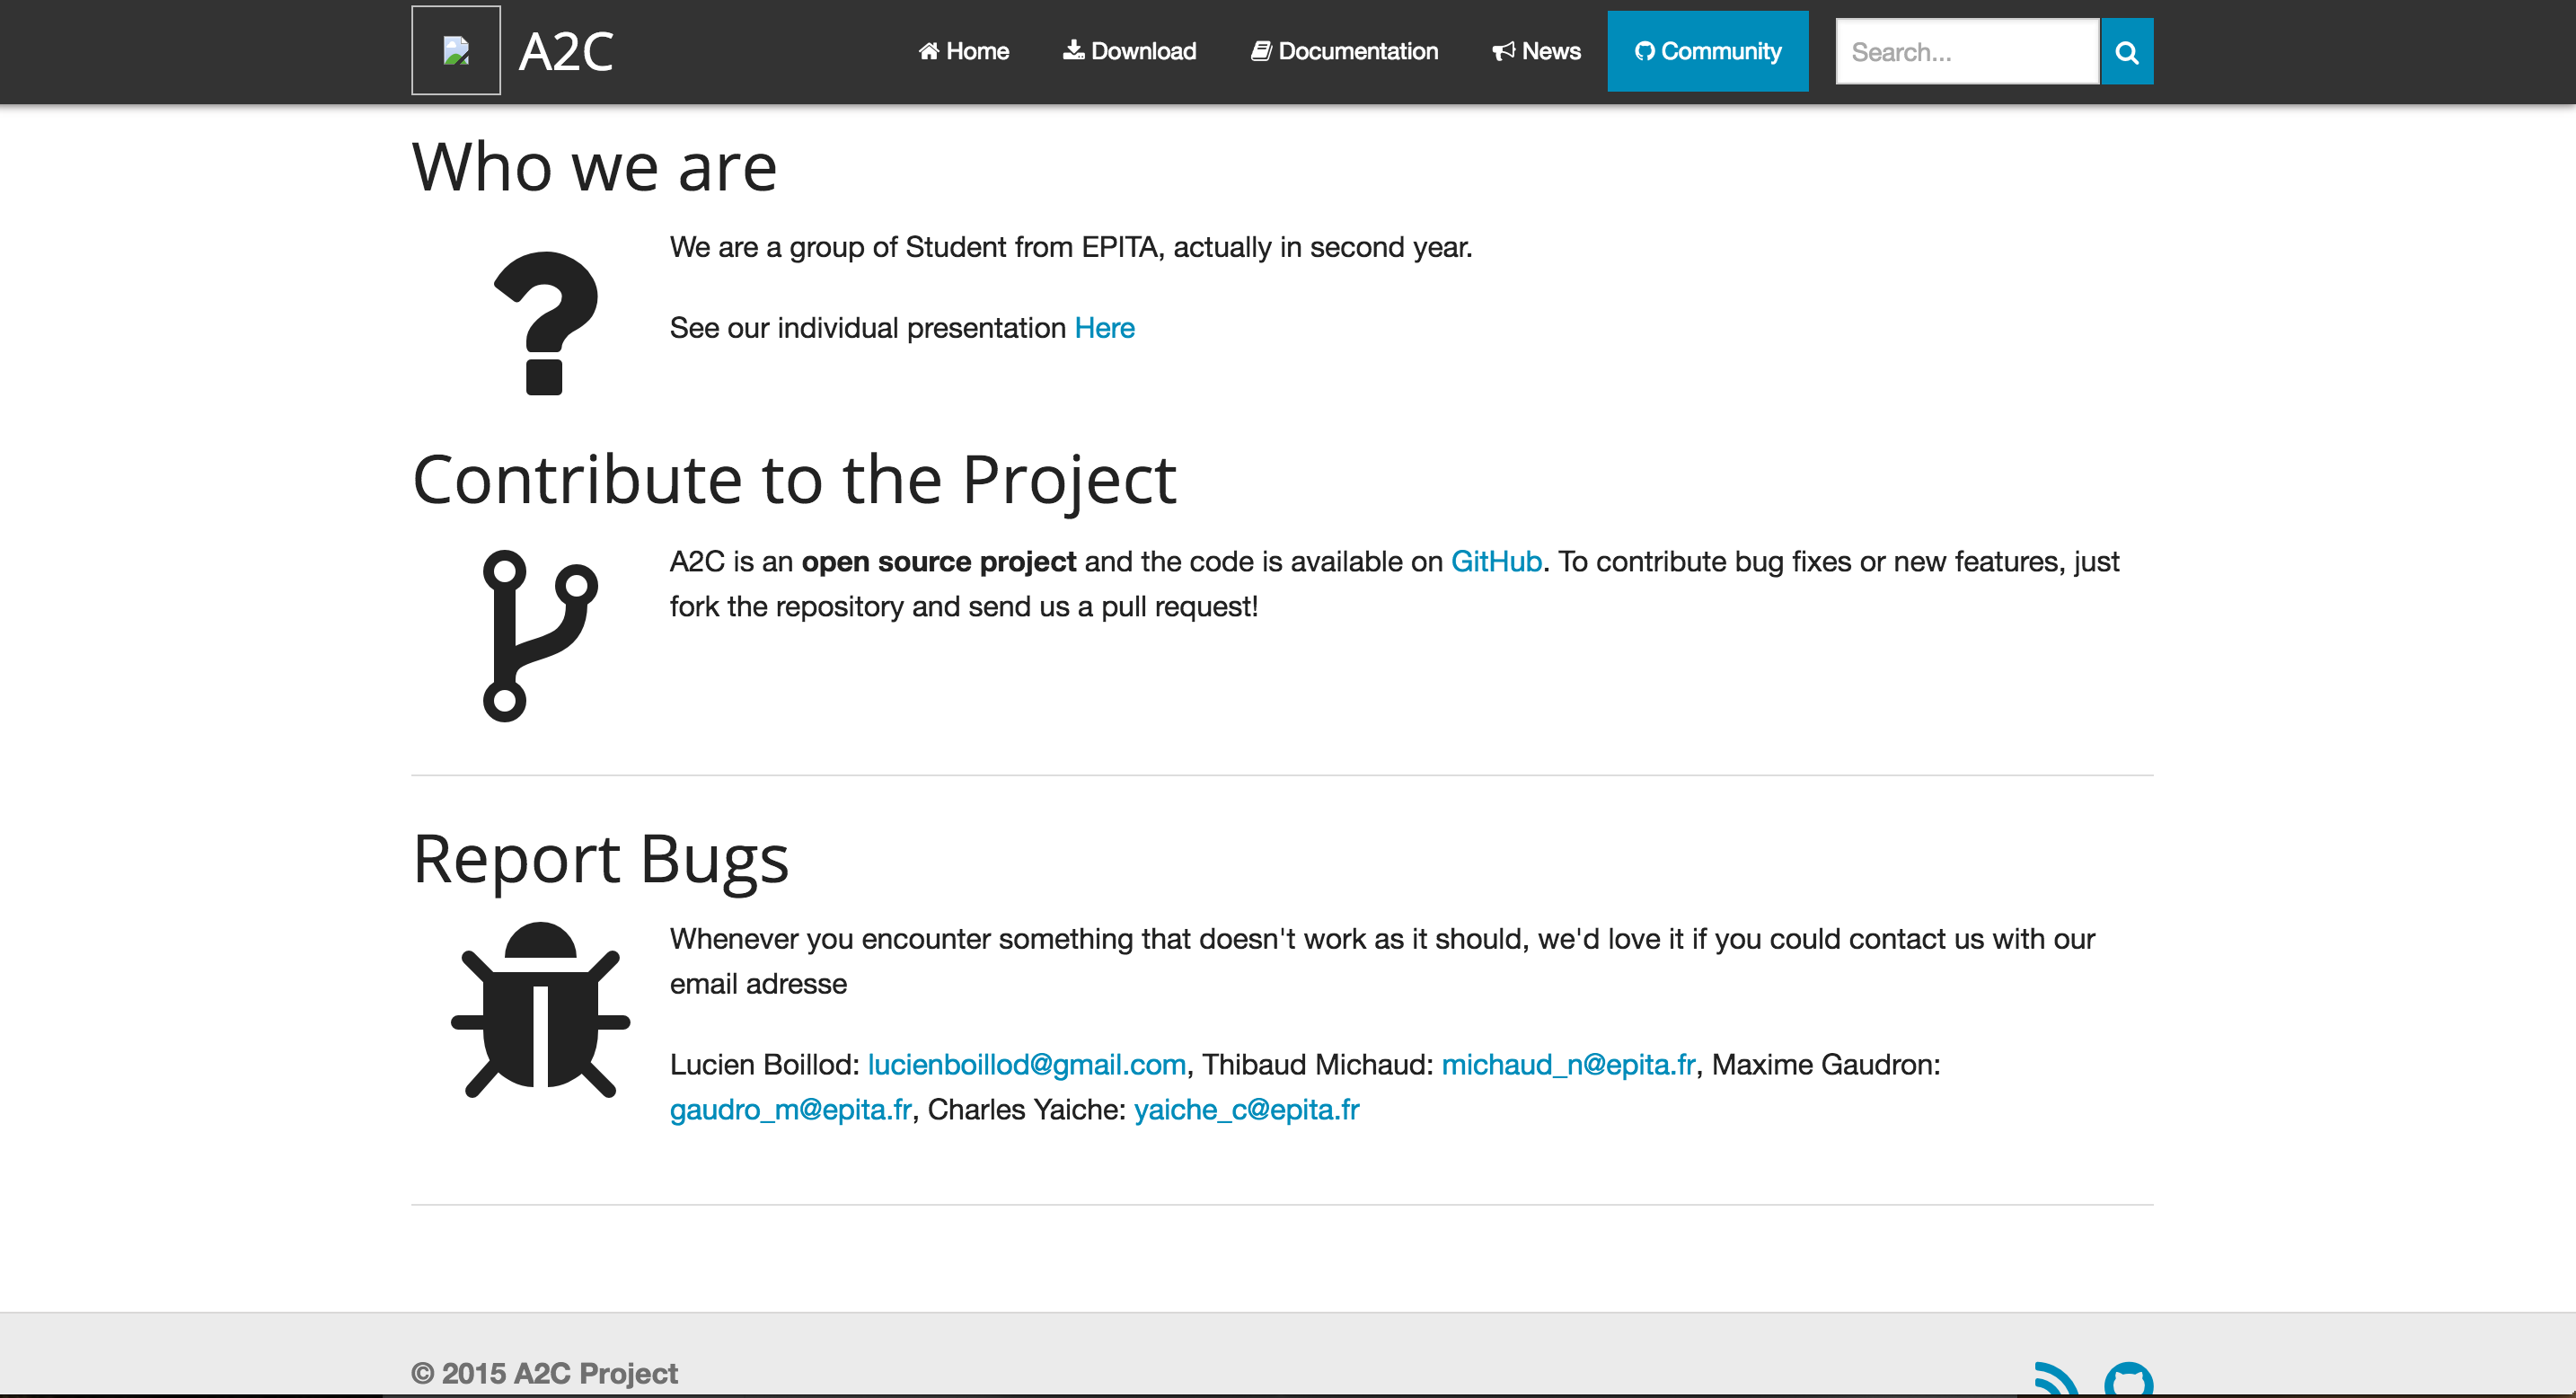
\includegraphics[scale=0.2]{website3.png}~\\[1.5cm] \\
\caption{Section contact}
\end{figure}

\newpage

\mychapter{3}{Rappels}
\section{Respect du cahier des charges}

Rappel du cahier des Charges

\begin{center}
\begin{tabular}{|c|c|c|c|}
\hline
                        & première soutenance & deuxième soutenance \\ \hline
site web                & done                & done                \\
\hline
structure de données     & done                & done                \\
\hline
lexer                   & done                & done                 \\
\hline
construction grammaire   & 75\%                & done                \\
\hline
parseur                 & 75\%                & done                \\
\hline
analyse sémantique      & 0\%                 & 25\%               \\
\hline
génération de code      & 0\%                 & 0\%                 \\
\hline

\end{tabular}
\end{center} \hfill 

Nos objectifs ont quelque peu été modifiés, au vu de nos choix d'implémentation et d'organisation. Cependant même si on se base sur les objectifs du cahier des charges on peut clairement voir qu'ils ont été remplis et dépassés. 

\begin{itemize}
\item site web : terminé et en ligne
\item structure de données : toutes les structures nécessaires au projet ont été implémentés. Cependant si besoin est, d'autres pourront être ajoutées.
\item lexeur complètement terminé et fonctionnel
\item construction de la grammaire : la grammaire abstraite est terminée (elle n'a pas d'autre intêret que de facilité la compréhension), et la grammaire implémentée est fini à 90\% puisqu'il reste uniquement à compléter l'en-tête des algos et rajouter les boucles.

\item parseur : lui aussi est terminé à 90\%, il doit avancer au même rythme que la grammaire.
\item analyse sémantique : 	10\% ont été réalisés, ce qui permet uniquement de vérifier les types des opérateurs unaires.
\item génération de code: 80\%, cette partie a bien avancée.
\end{itemize} 

Les objectifs ont donc été parfaitement remplis, voir bien plus. Le projet avance bien et un rendu est déjà disponible, ce qui permet d'avoir un projet stable auquel l'on rajoute des fonctionnalités. La base du projet est donc terminée.
\newpage

\section{Avance par rapport au cahier des charges}
Comme nous l'avons vu une certaine avance a été prise par rapports aux objectifs initiaux.
Comme on peut le voir, malgré la modification sur l'organisation du projet, ce dernier a avancé beaucoup plus rapidement et nos objectifs ont été plus que confirmés. Cela peut s'expliquer par les choix d'organisation que l'on a pris, autant au niveau de la fréquence de codage, que du choix d'avancer toutes les parties en même temps, plutot que d'en finir une avant d'en commencer une autre. Non seulement le travail parallèle est plus efficace mais il permet d'avoir un rendu assez rapidement, que l'on étoffe au fur et à mesure. \\

conclusion des tâches en avance:
\begin{itemize}
\item grammaire (+)
\item parseur (+)
\item generation de code (+++)
\item analyse sémantique (+)
\end{itemize}

\section{Ce qui reste à faire}

La plus grosse partie du travail se portera maintenant sur l'analyse sémantique, qui n'a à peine débuter. D'autre part on va étendre le langage pour arriver sur une couverture totale du langage Algo.

\subsection{2e soutenance}
\subsubsection{Grammaires}
La grammaire devra avancer en même temps que le parseur, puisque maintenant que nous avant quelque chose de fonctionnel sur un sous langage, l'objectif est d'aggrandir ce langage.
\subsubsection{Parseur}
Il faut aggrandir le langage, en ajoutant les boucles, les paramètres, les fonctions avec une valeur de retour, l'en tête de fonction, gestion de plusieurs fonctions dans un même fichier ... 
\subsubsection{Analyse sémantique}
Etant donné que le parseur est presque fini, il reste surtout la phase d'analyse sémantique à compléter. Voici une liste de points à implémenter d'ici la prochaine soutenance :
\begin{itemize}
\item finaliser l'analyse de type pour les structures plus complexe que les expressions arithmétique.
\item conception de la table des symboles.
\item gestion des contextes dans les algos (vérifier les portées des variables).
\item lier la définition d'une variable à son utilisation : il faut vérifier que l'utilisation d'une variable correspond à sa définition (et vérifier qu'elle a bien été définie), que l'on ne déclare pas plusieurs fois la même variable, etc.
\item vérifier que les expressions dans les conditions des structures de contrôle sont bien des expressions booléennes.
\end{itemize}
\subsubsection{Génération de code}
Pour la génération de code, pour l'instant nous laissons le choix à l'utilisateur quant à l'utilisation du code généré, mais biensur l'objectif et de sortir proprement un fichier C qui peut être compiler à la main ou de manière automatique. De plus et tout comme les autres tâches, il devra géré l'avancé du langage et généré le code équivalent en C.
\subsubsection{site web}
% finir parseur
% typecheking amélioré : gestion des types définis dans l'en-tête, checker les instructions (e.g. assignation d'une variable avec le mauvais type)

Concernant le site web, une documentation beaucoup plus fournie va être ajoutée, comme un wiki. La description des membres du groupe sera bientot complétée, ainsi que l'ajout du logo. Des news resteront postés de manières régulière afin de prévenir de l'avancement du projet et de ses releases.
\newpage

\subsection{3e soutenance}
% finir typechecking
% finir analyse sémantique
% - portée des variables (variables globales vs variables locales)
\epigraph{Everything has to be done}

\begin{center}
\begin{tabular}{|c|c|c|c|}
\hline
                         &dernière soutenance \\ \hline
site web                & done                                \\
\hline
structure de données     & done                               \\
\hline
lexer                   & done                                \\
\hline
construction grammaire   & done                               \\
\hline
parseur                 & done                             \\
\hline
analyse sémantique      & done                                \\
\hline
génération de code      & done                               \\
\hline

\end{tabular}
\end{center} \hfill 


\mychapter{4}{Conclusion}

On est très content du demarrage du projet. On a su former une structure solide et se poser les bonnes questions quant à l’implementation du projet. Le fait que l'on ai beaucoup réfléchi avant de coder a permis une implémentation efficace, on a donc réussi a trouver un bon compromis entre tout recoder "from sratch", et avancer dans le projet, notamment avec le parseur qu'on a finialement généré avec bison. Tous ces choix nous permettent d'avoir un projet fonctionnel sur un sous langage, que l'on étoffera au fur et a mesure de l'avancement du projet.

\newpage

\mychapter{5}{Sources}
\section*{Livres}
\noindent Compiler: Principles, Techniques and Tools (Dragon Book) \\
Modern Compiler Implementation in ML \\
\section*{Website}
\noindent http://www.google.com (meilleur ami) \\
http://stackoverflow.com \\
http://llvm.org \\
\section*{Autre}
\noindent Tyger Project d'EPITA (ING1) \\
Interpréteur de Marwan


\end{document}